\documentclass[crop,tikz]{standalone}% 'crop' is the default for v1.0, before it was 'preview'
\usepackage{tikz,calc,pgfplots}
\usetikzlibrary{calc,patterns}
\begin{document}
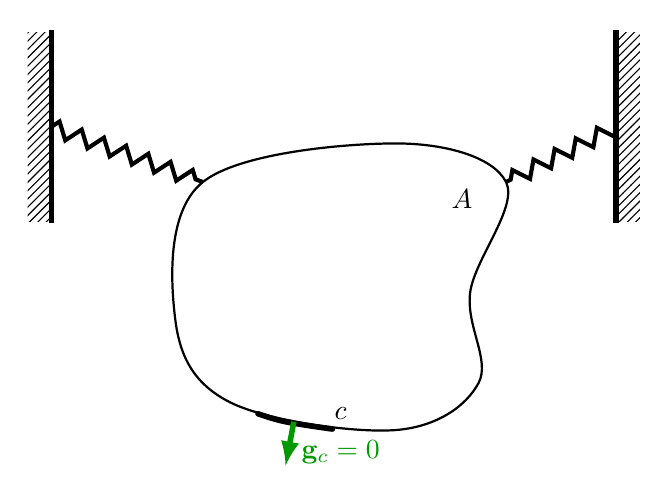
\begin{tikzpicture}[scale=0.7]

\draw [thick]  plot[smooth cycle, tension=.6] coordinates {(0,2) (0.5,4.5) (4,5.2) (6,4.5)  (5.35,2.5) (5.5,0.85) (4,0) (1,0.5) };
\node[outer sep=0pt,thick] at (5.2,4.2) [] {${A}$};



\draw [line width=2pt,black,cap=round]  plot[smooth, tension=.6] coordinates { (2.85,0.0175) (2,0.15) (1.5,0.295) };  
\node[outer sep=0pt,thick] at (3,0.3) [] {$c$};


\draw [line width=2pt,black!40!green,solid,latex-] plot[] coordinates { (2.0,-0.65)  (2.15,0.15) }; 

\node[outer sep=0pt,thick] at (3,-.4) [black!40!green] {{$\mathbf{g}_{c}=0$}};


\draw [line width=2pt,black,solid,-] plot[] coordinates { (-2.25,3.75)  (-2.25,7.25) }; 

\tikzstyle{ground}=[fill,pattern=north east lines,draw=none,minimum height=0.3cm,inner sep=0pt,outer sep=0pt]

\node (ground) [ground,anchor=south,minimum width=2.4cm,rotate = 90] at (-2.25,5.5) {};

\node (ground) [ground,anchor=south,minimum width=2.4cm,rotate = -90] at (8,5.5) {};
\draw [line width=2pt,black,solid,-] plot[] coordinates { (8,3.75)  (8,7.25) }; 

\draw[decoration = {zigzag,segment length = 3mm, amplitude = 1mm},decorate,line width = 1.5pt] (-2.25,5.5)--(0.5,4.5) node [above,left,xshift=3.75cm,rotate = 0, yshift = 0.85cm,align=center] {};
\draw[decoration = {zigzag,segment length = 3mm, amplitude = 1mm},decorate,line width = 1.5pt] (8,5.5)--(6,4.5) ;

	

\end{tikzpicture}
\end{document}
